\section{Detector description}
\label{sec:detector}

\begin{center}
  \fbox{\begin{minipage}{\linewidth}
    To check:
    \begin{itemize}
      \item bias voltage levels on the wire planes
      \item grounding
      \item the general description of the connections
    \end{itemize}
  \end{minipage}
  }
\end{center}

The ICARUS detector includes two modules (\ICARUSmodule), each with two \TPC's
sharing the cathode, which will be kept at a potential of \kiloV{-75}.
Each TPC anode is made of three wire planes (\cref{fig:WireCategories}),
which are kept at a potential close to the ground.
The first one, commonly called first induction plane, has horizontal wires, each
about 10 meters long and spanning half of the detector, and kept at \V{-300}.
Each half plane includes 1056 channels, all ending on the sides of the anode
plane frame.
Three millimeters away, the second plane (``second induction plane'') is made of
wires at an angle of $\pi/6$ from the vertical ($\pi/3$ from the horizontal
wires) at ground (\V{0}).
Its wires can be grouped in three sets: the longest ones, terminated on the top
and on the bottom of the anode plane frame\footnote{%
The wires are spaced at $d=\mm{3}$, and their terminations are spaced at
$2/\sqrt{3}\,d=\mm{3.46}$.%
},
the shorter ones that terminate on the bottom and on the side of the anode
frame, and the shorter ones that terminate on the top and on the side of the
frame.
Located other \mm{3} away, the third plane (``collection plane'') is similar to
the second induction plane, but with angle $\pi/6$ of the other side of the
vertical, and at \V{300}. Its wires follow the same categories.
\begin{figure}
  {
    \centering
    % trimming to remove some residuals of the wires on the sides
    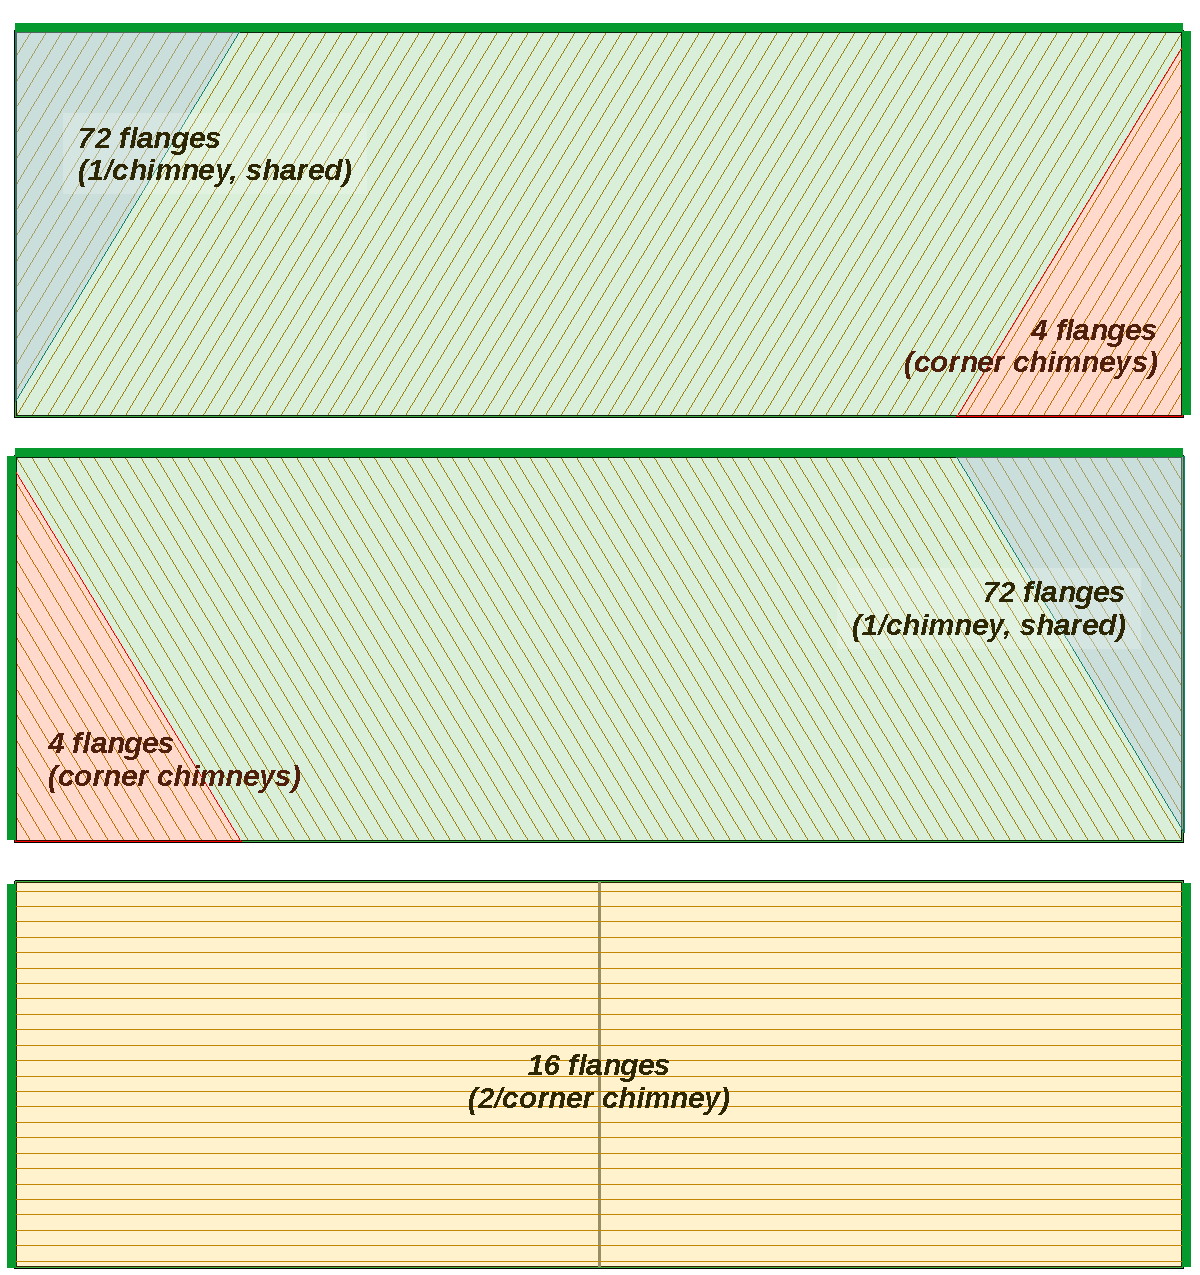
\includegraphics[height=11cm,clip,trim=1 0 1 0]{fig/WireCategories}\\
  }
  \caption{
    The wires in a single TPC (not in scale!) coded by category. The top plane (\emph{collection}) and middle plane (\emph{second induction}) feature three different categories of wires: side-to-bottom \emph{(in red)}, top-to-bottom \emph{(in green)} and top-to-side \emph{(in blue)}, while the last plane (\emph{first induction}) has middle-to-side wires \emph{(in yellow)}. The thick green borders represent the sides where the TPC wires are connected to the 68-wire cables.
  }
  \label{fig:WireCategories}
\end{figure}
\\
At the top termination, or at the side termination if no top one is present,
the wires are pinned in groups of 32 on a board (\emph{Comb-to-Cable Interface},
CCI) and their signal conveyed to a 68 pin connector.
Each board is about \cm{11} long ($32 \times \mm{3} / \cos \pi/6$) on the top
frame.
The connector hosts a twisted pair cable, with 34 pairs of wires, one in each pair
connected to the wire and carrying the signal, and the other twisted around the
former to shield it from interference. The highest two pairs (number 33 and 34)
of the cable are not used for transmission of signal.
In the final configuration of the detector, shield wires are grounded via the
readout boards, but in the detector configuration at time of the test readout
boards are not present yet and the shield wire electric potential is expected to
be floating.
It became evident in the previous connectivity test that, regardless the design
intentions, some of the shield wires are actually grounded to the detector,
while others are not grounded. This feature has been confirmed by previous
observations from the time when the detector was being refurbished at CERN.
All the cables are cut to be of the same length, resulting into the ones to the
closest wires having a lot of spare length, and into the ones to the farthest
wires having little to none.\\
Cables from the top of the anode frame are tied in bundles of 18, half from the
second induction and half from the collection plane, to pass through a
``chimney'' with a single flange (``top chimney'').
Likewise, cables from the sides are also bundled, two bundles collecting all the
33 first induction plane cables (bundles of 18 and 15 cables) and another bundle
collecting the 18 from the other plane, and lead to one of the tall chimneys at
the ends of the modules (``corner chimneys'') featuring three flanges each.\\
At the flange, the 18 cables are connected to decoupling and biasing
boards\cite{ICARUSDBB} (\DBB, \cref{fig:DBB}).
In the top flanges that host cables from two different planes, each one of the
nine boards on a single flange serves a cable from the second induction plane
and one from the collection plane.
Its purpose is twofold: to deliver the bias voltage of the wire plane, and
to convey the induced current as a potential for the front end to read
(removing the bias voltage via a \nanoF{10} capacitor).
The board is split into two insulated halves: each can serve a
different plane with a different bias voltage.
For its physical characteristics, the two halves are sometimes referred to as
long (or tall) and short; in the blueprints, they are called \emph{left} (L)
and \emph{right} (R), respectively.
The two sides are identical, both functionally and component-wise, but they are
insulated from each other because of the different bias voltage they have to
distribute.
In addition to some circuitry common to all channels within a half board, each
channel also has its own dedicated circuitry, independent and insulated from
the other channels.
\begin{figure}
  \subfloat[]{
    \label{fig:DBB}
    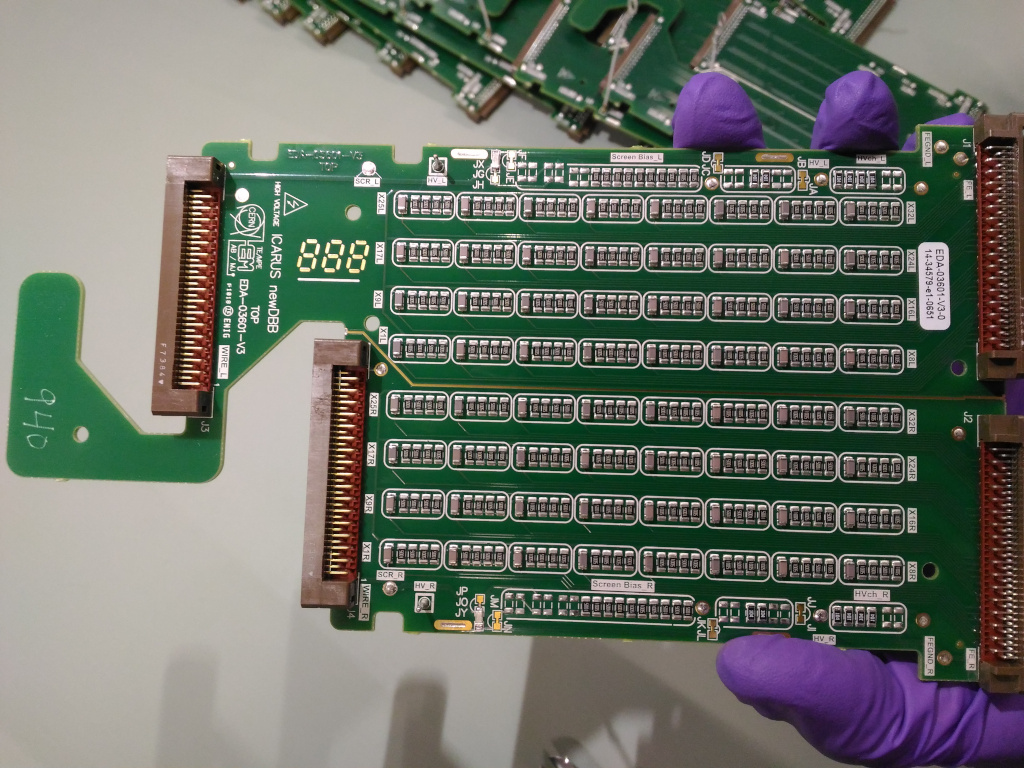
\includegraphics[height=6cm]{fig/20181201-171653_DBB}
  }
  \subfloat[]{
    \label{fig:AssembledFlange}
    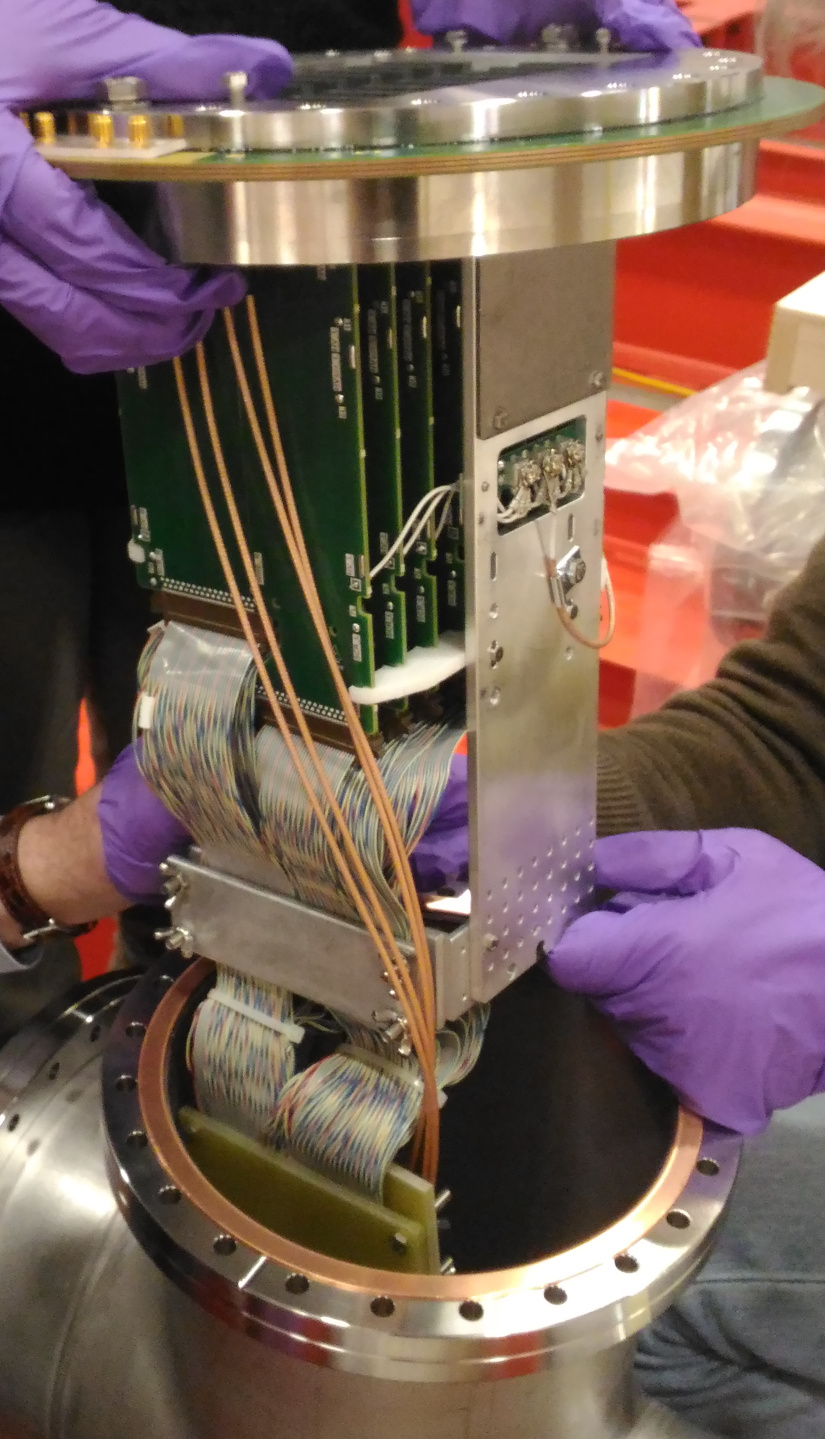
\includegraphics[height=6cm]{fig/20181218_173444_flange}
  }
  \caption{
    \protect\subref{fig:DBB}
      a decoupling and biasing board;
    \protect\subref{fig:AssembledFlange}
      a flange with nine \DBB's being positioned back into its chimney.
    The four golden cables connect to the test capacitance at the bottom of the
    anode frame. On the right side, the distribution of bias voltage can be
    seen, from a single cable into three and then nine channels to the long side
    of each DBB via white wires.
  }
\end{figure}
The \DBB offers four connectors: two are 68-pin connectors with clips, which
host the cables from the wires, one side for each plane.
The others, also one per board side, plug directly into the flange.
In addition, the board has two wires, also one per side, to be connected to the
bias voltage distribution on the flange frame.
\begin{figure}
  % TODO add a picture of a real flange
  \centering
  \subfloat[Flange and test setup with minicrate.]{
    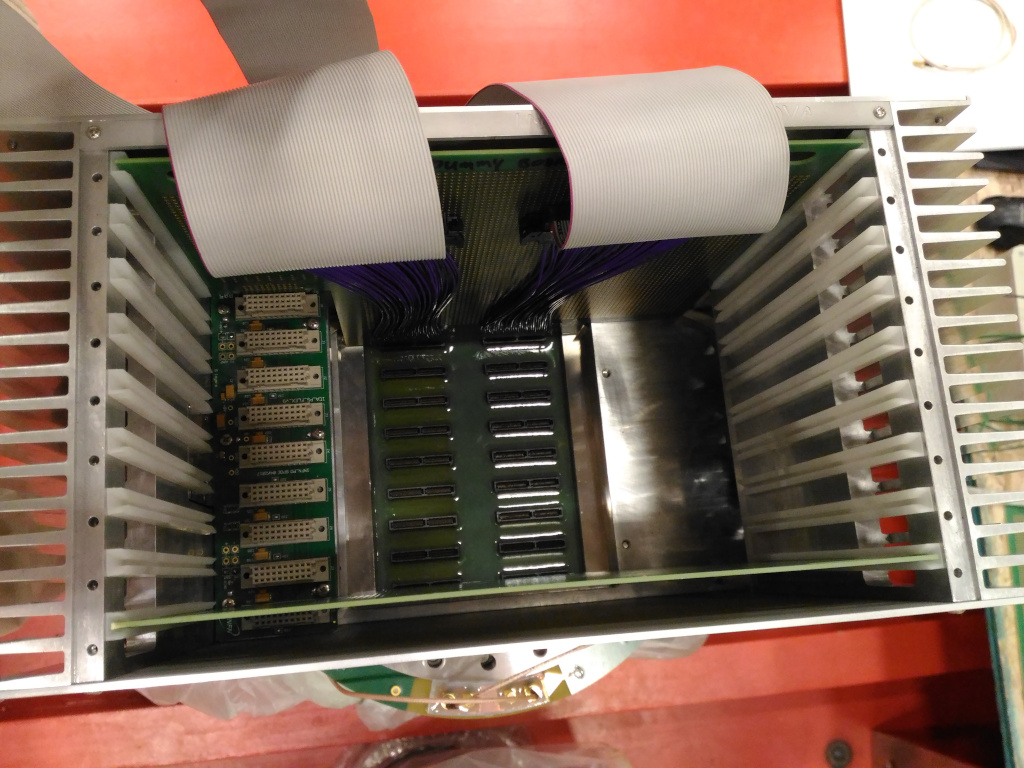
\includegraphics[height=4cm]{fig/20181201_165211_TopFlangesAndMinicrate}
    \label{fig:MinicrateSetup}
  }
  \subfloat[Flange connection conventions.]{
    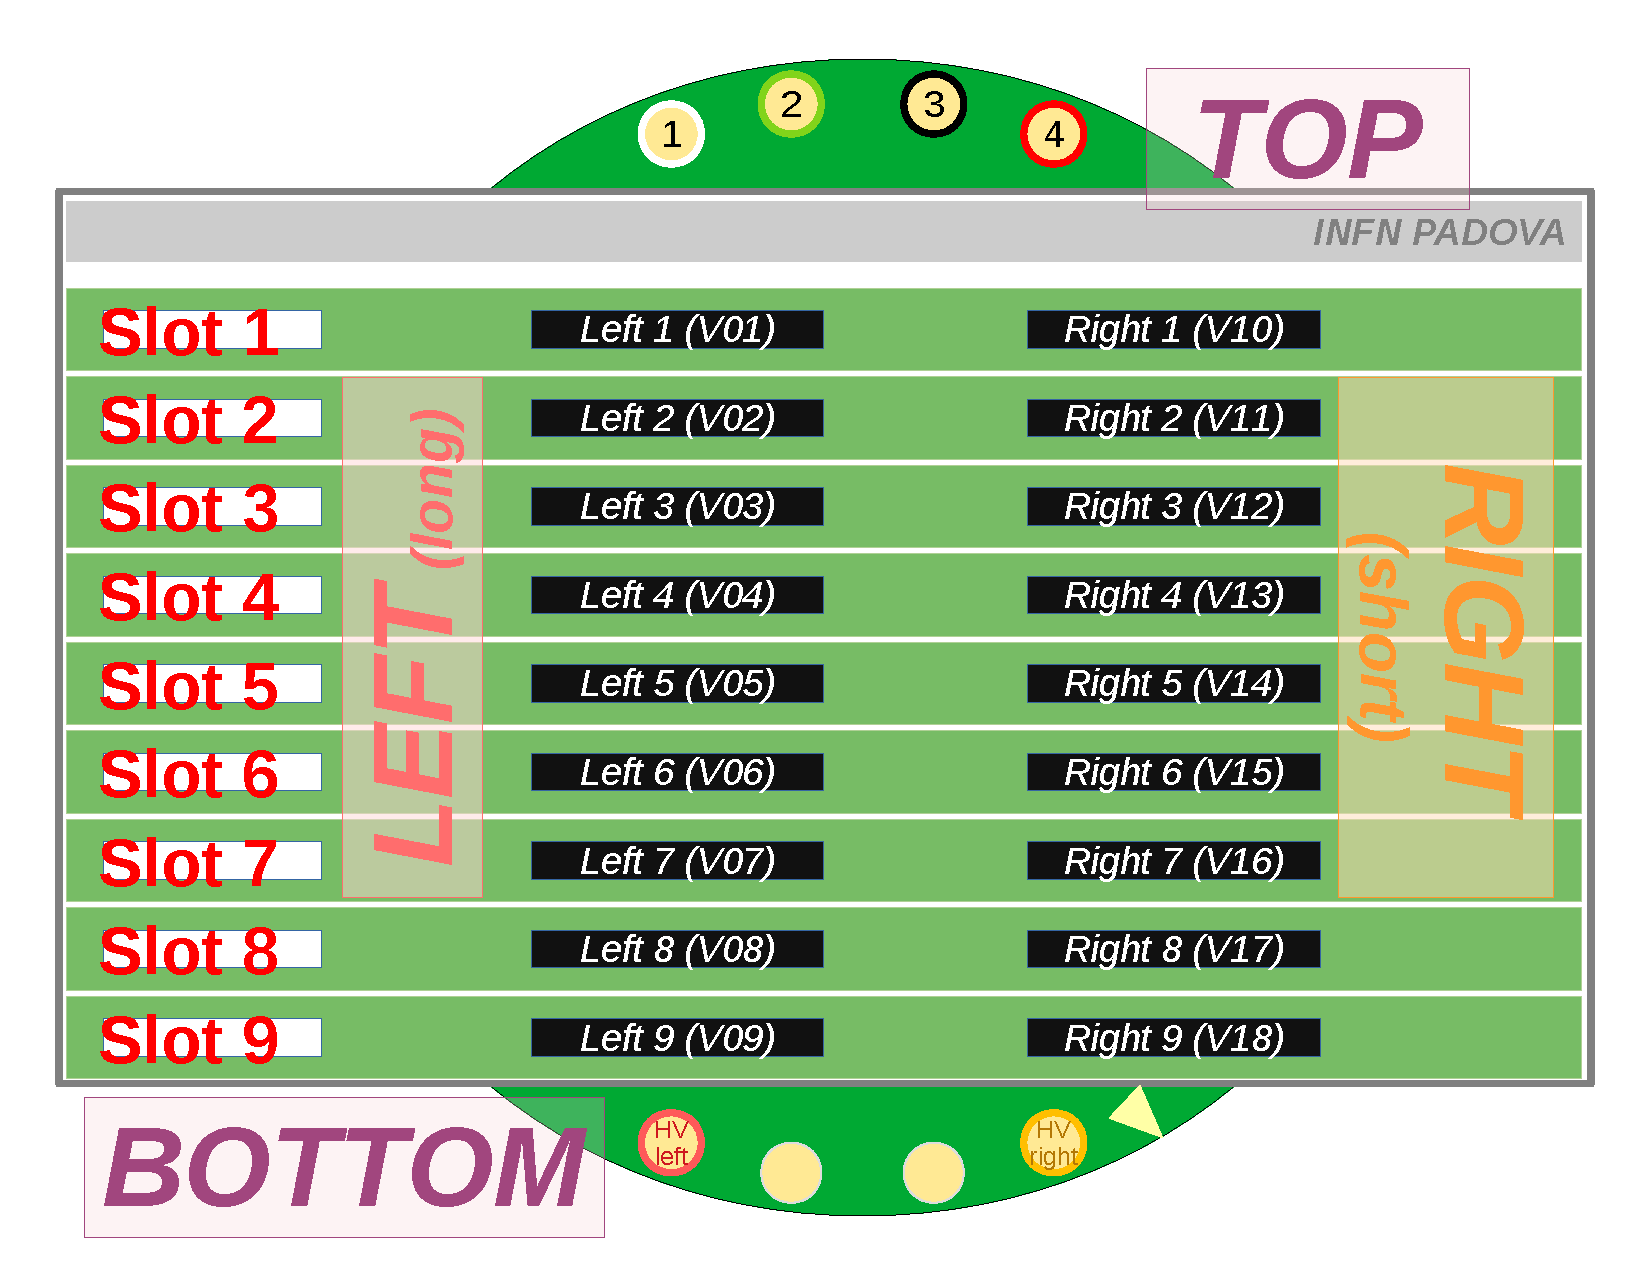
\includegraphics[height=5cm]{fig/TopFlangesAndMinicrate}
    \label{fig:FlangeConnections}
  }
  \caption{
    \protect\subref{fig:MinicrateSetup}
      Test set up with a readout minicrate mounted on a flange of a top chimney,
      plus test board, and
    \protect\subref{fig:FlangeConnections}
      illustration of the external connections of a flange with the nomenclature
      conventionally used during the connectivity test.
    \\
    The triangular marking (at the bottom right of the flange) sets the orientation.
    The test pulse cables used to be referred to with color tags, and we'll keep
    that tradition for consistency (see \cref{ssec:labelling}).
  }
\end{figure}
A flange is the interface between the cold environment inside the cryostat and 
the outside, warm environment, where the front end readout is.
It exposes nine pairs of connectors (each backed by a single \DBB), and four SMA
connectors (wire female, shield male) on each of two sides.
Of the two sets of four, the bottom one (defined as in
\cref{fig:FlangeConnections}) hosts the distribution channel of bias voltage for
the left side of the \DBB's on the leftmost connector, and for the right side on
the rightmost connector, while the central ones are unused.
The set on the top of the flange hosts the four cables distributing the test
pulses to the wires connected to the bottom of the anode frame, which we'll
describe next.
\\
The termination boards on the bottom of the anode frame feature a test capacitor
of sorts (\cref{fig:TestCapacitance}), where the dielectric material is
the board itself, and the electrodes are the terminating wire on one side, and a
band of deposited conductor on the other, which spans all 32 wires.
\begin{figure}
  \center
  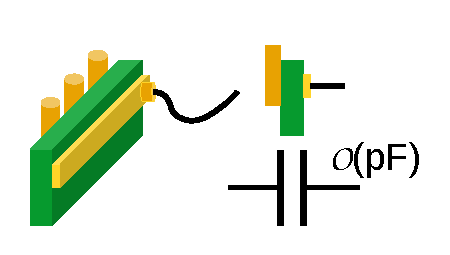
\includegraphics[height=2.5cm]{fig/TerminatorCapacitance}
  \caption{\label{fig:TestCapacitance}
    Illustration of the path for the test pulses from the flange to the wires.
  }
\end{figure}
This band can be connected to a cable for injecting test pulses.
When doing so, a signal, differentiation of the test pulse, is induced on all
the wires, from which it can be read via readout or via a specific testing
setup.
There are four test pulse cables departing from each flange to serve the 18
cables (576 wires) the flange connects to (\cref{fig:PulseCables}).
Two cables are connected to the second induction plane, while the other two are
connected to the collection plane.
\begin{figure}
  \center
  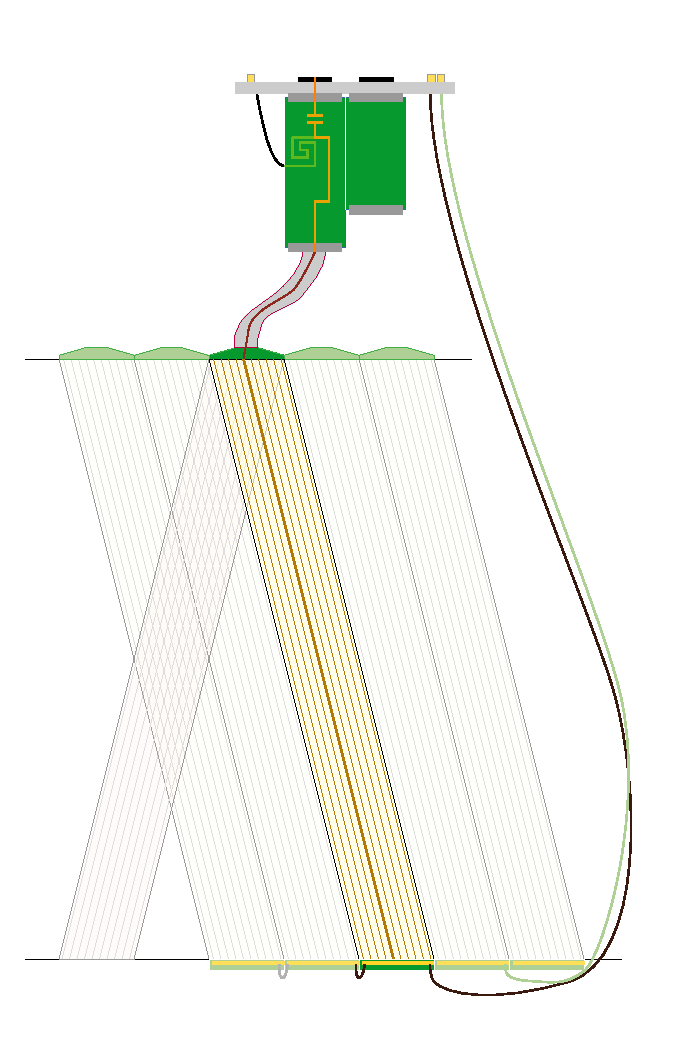
\includegraphics[height=10cm]{fig/PulseCablePath}
  \caption{\label{fig:PulseCables}
    Illustration of the path of test pulses from the flange to the wires and
    back to the front-end
    (see \cref{sec:methodology} for more details).
  }
\end{figure}
The general rule is that one of the two cables is connected to a daisy chain of
eight termination boards, while the remaining one serves a single board
(\cref{fig:TestPulseDistribution}).
\begin{figure}
  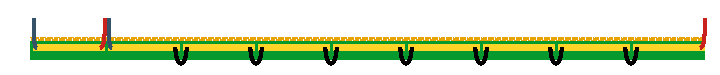
\includegraphics[width=\textwidth]{fig/TerminatorDaisyChain}
  \caption{\label{fig:TestPulseDistribution}
    Distribution of the test pulse to the boards with the test capacitance.
  }
\end{figure}
This rule has been observed to have quite some exceptions (see
\cref{fig:PulseCableMap}).
The cables themselves have been color-tagged, but that tag is not visible from
the outer side of the flange: instead, a convention is followed as illustrated
in \cref{fig:FlangeConnections}.
While swapping bias voltage cables would have catastrophic effects, swapping
test pulse cables has little to no effect beside adding some confusion, since
the colors are purely conventional.
These flanges are spread across the length of the detector, one per chimney,
in four columns each one roughly above one of the anodes, with the exception
of the end chimneys which will be described shortly.
On top of the flange, a minicrate with VME bus will be mounted
(as in \cref{fig:MinicrateSetup}), hosting nine readout boards into as many
slots, with each one matching a single \DBB.
\\
The description above reflects the installation of wires terminated at the top
of the anode frame.
That includes all the full length wires from second induction and from
collection planes, plus the half among the shorter ones which are terminated at
top (green and blue categories in \cref{fig:WireCategories}), and it leaves out
the other half of the shorter wires on those planes (red in that figure), plus
all the wires from the first induction plane (yellow in that figure), 
all of which are terminated on the sides of the frame.
To read out these wires, their cables (with different length) are brought up to
the chimneys at the end of the detector (rows 1 and 20).
These chimneys are special in that they stack three flanges instead of hosting
just one: the top two serve the first induction plane
(\cref{fig:HorizontalWireChimney}), and the bottom one serves the shorter
wires\footnote{%
These wires all belong to the same plane, either second induction or collection.
The shorter wires from the other plane terminate on the top and they are served
by a different chimney.
}
and they have no connection to test pulse cables.
They still have two bias voltage lines, which may be connected to any of the
four SMA connectors. None of these wires is provided with a test capacitor,
therefore the test pulse connectors are disconnected.
\begin{figure}
  {
    \centering
    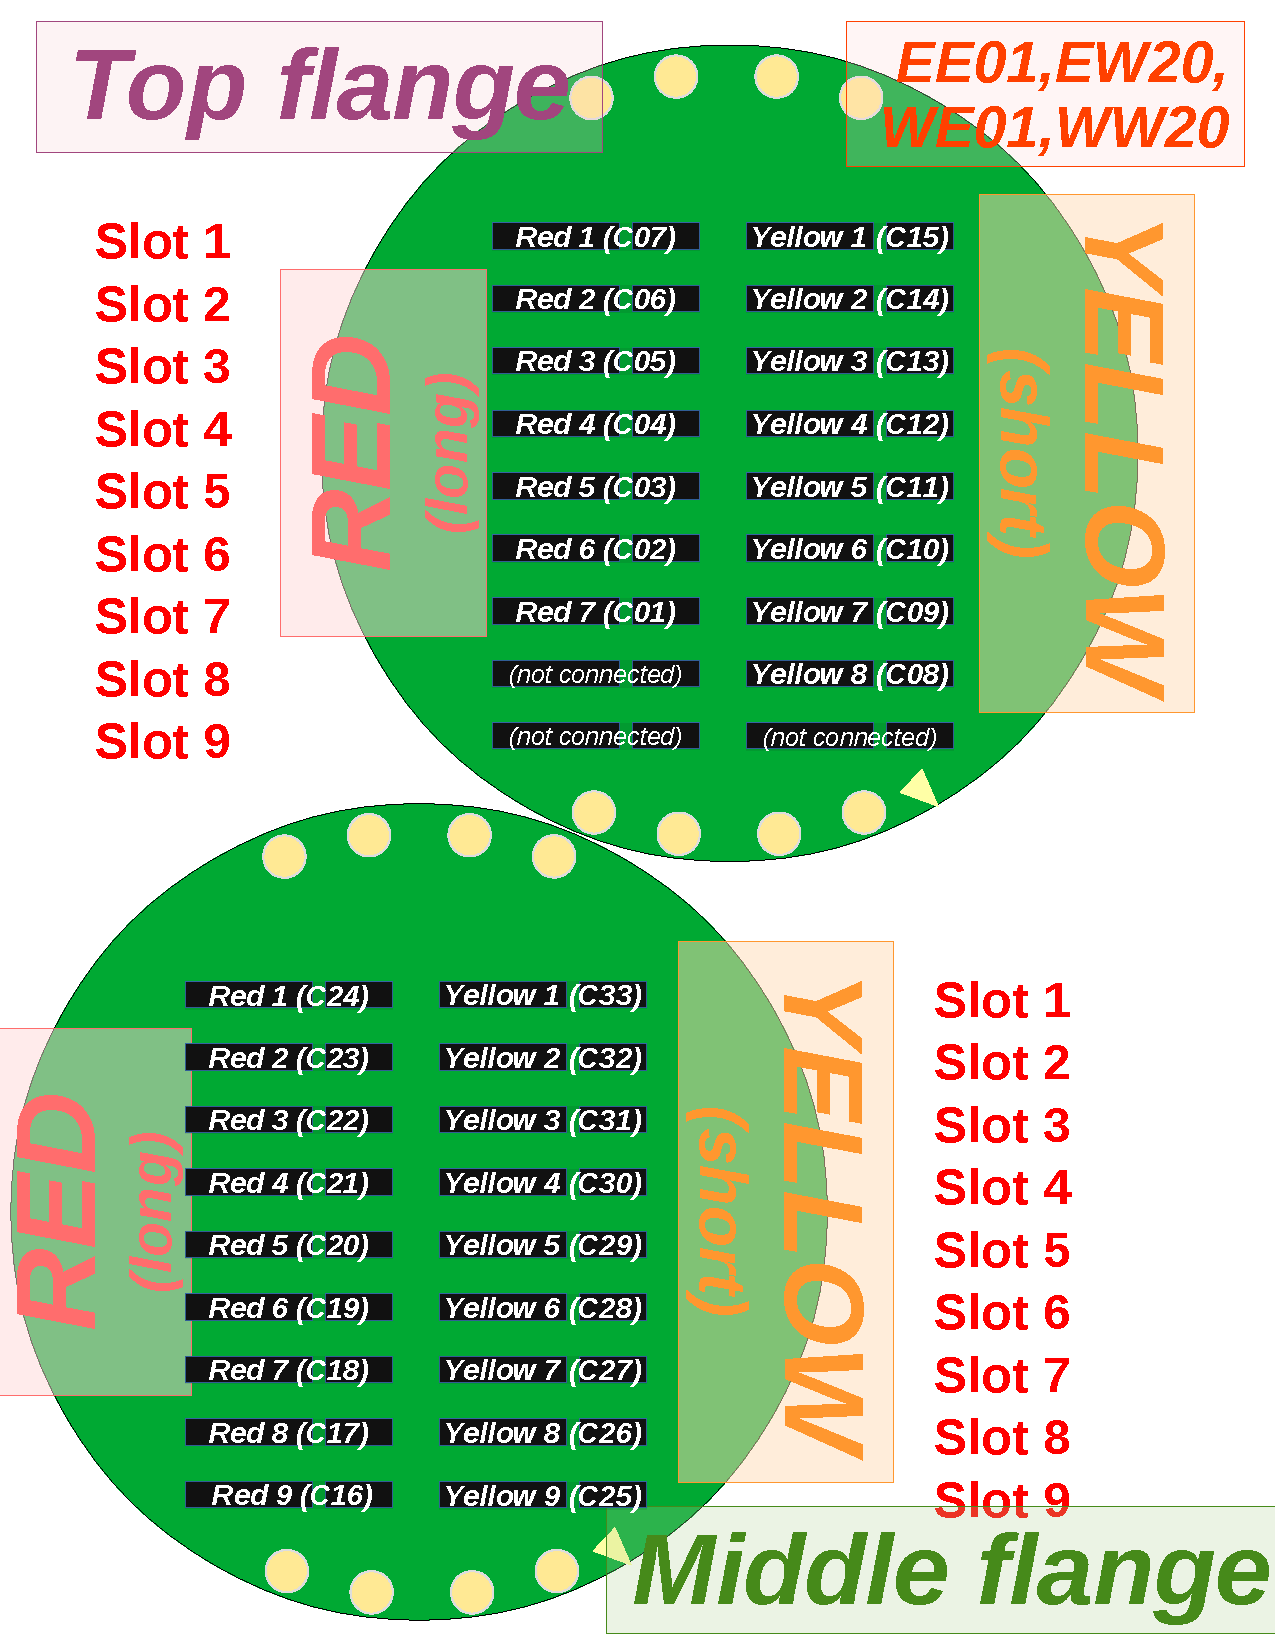
\includegraphics[width=\textwidth]{fig/CornerFlanges}
    \\
  }
  \caption{\label{fig:HorizontalWireChimney}
    Illustration of the external connections of the flanges serving horizontal
    wires.
    The triangular marking sets the orientation.
    Due to the relative orientation, the ``left'' and ``right'' labeling becomes
    confusing, and we resort to an arbitrary color coding instead.
  }
\end{figure}
The number of wires on first induction plane, 1054, requires 33 connectors with
32 channels each.
Since all the flanges are standard, they have 18 connectors each.
As a consequence, of the two flanges dedicated to that plane, one has three
connectors not connected to any wire.
Due to readout bus requirements, a ``master'' board always needs to be plugged
into the first ``slot'', and for this reason it was chosen to always have a
fully connected \DBB in the first slot of each flange.
\\
Most of the components are physically keyed to prevent mounting them in any but
the right way.
That includes the minicrates (with different step on the top and bottom screw
holes), the slots (with a shorter and a longer side), the 68 pin connectors,
and also the connectors on the flange to the readout board (each split into a
shorter and a longer side).
The SMA connectors, instead, are not keyed nor marked in any way, and
conventions need to be followed to identify each of them.

